\documentclass[10pt]{article}\usepackage[]{graphicx}\usepackage[]{color}
%% maxwidth is the original width if it is less than linewidth
%% otherwise use linewidth (to make sure the graphics do not exceed the margin)
\makeatletter
\def\maxwidth{ %
  \ifdim\Gin@nat@width>\linewidth
    \linewidth
  \else
    \Gin@nat@width
  \fi
}
\makeatother

\definecolor{fgcolor}{rgb}{0.345, 0.345, 0.345}
\newcommand{\hlnum}[1]{\textcolor[rgb]{0.686,0.059,0.569}{#1}}%
\newcommand{\hlstr}[1]{\textcolor[rgb]{0.192,0.494,0.8}{#1}}%
\newcommand{\hlcom}[1]{\textcolor[rgb]{0.678,0.584,0.686}{\textit{#1}}}%
\newcommand{\hlopt}[1]{\textcolor[rgb]{0,0,0}{#1}}%
\newcommand{\hlstd}[1]{\textcolor[rgb]{0.345,0.345,0.345}{#1}}%
\newcommand{\hlkwa}[1]{\textcolor[rgb]{0.161,0.373,0.58}{\textbf{#1}}}%
\newcommand{\hlkwb}[1]{\textcolor[rgb]{0.69,0.353,0.396}{#1}}%
\newcommand{\hlkwc}[1]{\textcolor[rgb]{0.333,0.667,0.333}{#1}}%
\newcommand{\hlkwd}[1]{\textcolor[rgb]{0.737,0.353,0.396}{\textbf{#1}}}%
\let\hlipl\hlkwb

\usepackage{framed}
\makeatletter
\newenvironment{kframe}{%
 \def\at@end@of@kframe{}%
 \ifinner\ifhmode%
  \def\at@end@of@kframe{\end{minipage}}%
  \begin{minipage}{\columnwidth}%
 \fi\fi%
 \def\FrameCommand##1{\hskip\@totalleftmargin \hskip-\fboxsep
 \colorbox{shadecolor}{##1}\hskip-\fboxsep
     % There is no \\@totalrightmargin, so:
     \hskip-\linewidth \hskip-\@totalleftmargin \hskip\columnwidth}%
 \MakeFramed {\advance\hsize-\width
   \@totalleftmargin\z@ \linewidth\hsize
   \@setminipage}}%
 {\par\unskip\endMakeFramed%
 \at@end@of@kframe}
\makeatother

\definecolor{shadecolor}{rgb}{.97, .97, .97}
\definecolor{messagecolor}{rgb}{0, 0, 0}
\definecolor{warningcolor}{rgb}{1, 0, 1}
\definecolor{errorcolor}{rgb}{1, 0, 0}
\newenvironment{knitrout}{}{} % an empty environment to be redefined in TeX

\usepackage{alltt}
\usepackage{amssymb, amsmath, amsthm, verbatim, layout, setspace, graphicx, float, geometry}
\usepackage{booktabs}

\newcommand{\textnote}[1]{\textbf{\textit{#1}}}
\newcommand{\code}[1]{\textbf{\textit{#1}}}
\newcommand{\grad}{\nabla}

% ------ layout ------
\IfFileExists{upquote.sty}{\usepackage{upquote}}{}
\begin{document}
\title{Linear Regression: Part 2}
\author{Jeremy Oldfather}
\maketitle







\subsection*{Multiple Linear Regression - Last Time }

When we regress $y$ on more than one independent variable, say ($x_1, x_2,...,x_k$) rather than simply ($x_1$), the regression framework is referred to as {\bf multiple linear regression}.

What might motivate us to introduce multiple regressors? One reason might be that we have reason to suspect {\bf omitted variable bias}. In order for our model to be subject to omitted variable bias, we must have both of the following problems:

\begin{description}
  \item [$E(y|x_1,x_2) \ne E(y|x_1) $] :  Meaning our expectation about the dependent variable $y$ changes when we include the additional independent variable. If $E(y|x_1,x_2) = E(y|x_1)$, we would say that $y$ is conditionally independent of $x_2$---meaning either $x_2$ is completely irrevelant to predicting $y$, or that any information contained in $x_2$ is already contained in $x_1$.
  \item [$Cor(x_1, x_2) \ne 0 $] :  Meaning the additional variable $x_2$ must be correlated with a current dependent variable $x_1$.
\end{description}

For example, when we plot the distribution of residuals from our previous model by neighborhood, we can see that the variable {\bf neighborhood} meets the first critera for omitted variable bias since for Anacostia we would consistently overstate the impact of a change in living area on the change in sales price.

\begin{knitrout}\small
\definecolor{shadecolor}{rgb}{0.969, 0.969, 0.969}\color{fgcolor}\begin{kframe}
\begin{alltt}
\hlstd{selected.nhoods}\hlkwb{<-}\hlkwd{c}\hlstd{(}\hlstr{"FOGGY BOTTOM"}\hlstd{,}\hlstr{"ANACOSTIA"}\hlstd{,}\hlstr{"LEDROIT PARK"}\hlstd{,}\hlstr{"TAKOMA"}\hlstd{,}\hlstr{"GEORGETOWN"}\hlstd{)}
\hlkwd{data.frame}\hlstd{(}\hlkwc{e}\hlstd{=}\hlkwd{resid}\hlstd{(fit),}\hlkwc{g}\hlstd{=data.model}\hlopt{$}\hlstd{neighborhood)} \hlopt
  \hlkwd{filter}\hlstd{(g} \hlopt \hlstd{selected.nhoods)} \hlopt
  \hlkwd{ggplot}\hlstd{(}\hlkwd{aes}\hlstd{(}\hlkwc{y}\hlstd{=e,}\hlkwc{x}\hlstd{=g))} \hlopt{+} \hlkwd{geom_boxplot}\hlstd{()}
\end{alltt}
\end{kframe}

{\centering 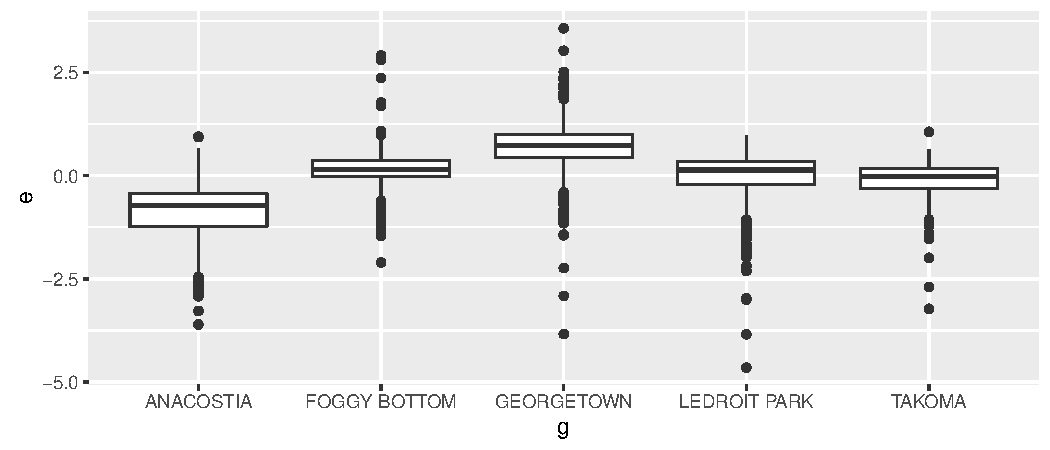
\includegraphics[width=\maxwidth]{figure/boxplot_residuals-1} 

}



\end{knitrout}

To check the second criteria, that $Cor(living\_area,neighborhood) \ne 0$, we can plug a dummy variable for each neighborhood into R's {\bf cor()} function.

\begin{knitrout}\small
\definecolor{shadecolor}{rgb}{0.969, 0.969, 0.969}\color{fgcolor}\begin{kframe}
\begin{alltt}
\hlkwd{cor}\hlstd{(data.model}\hlopt{$}\hlstd{log_living_sqft,data.model}\hlopt{$}\hlstd{neighborhood}\hlopt{==}\hlstr{"ANACOSTIA"}\hlstd{)}
\end{alltt}
\begin{verbatim}
## [1] 0.02040842
\end{verbatim}
\begin{alltt}
\hlkwd{cor}\hlstd{(data.model}\hlopt{$}\hlstd{log_living_sqft,data.model}\hlopt{$}\hlstd{neighborhood}\hlopt{==}\hlstr{"FOGGY BOTTOM"}\hlstd{)}
\end{alltt}
\begin{verbatim}
## [1] -0.1058928
\end{verbatim}
\begin{alltt}
\hlkwd{cor}\hlstd{(data.model}\hlopt{$}\hlstd{log_living_sqft,data.model}\hlopt{$}\hlstd{neighborhood}\hlopt{==}\hlstr{"GEORGETOWN"}\hlstd{)}
\end{alltt}
\begin{verbatim}
## [1] 0.06697943
\end{verbatim}
\begin{alltt}
\hlkwd{cor}\hlstd{(data.model}\hlopt{$}\hlstd{log_living_sqft,data.model}\hlopt{$}\hlstd{neighborhood}\hlopt{==}\hlstr{"LEDROIT PARK"}\hlstd{)}
\end{alltt}
\begin{verbatim}
## [1] 0.03272786
\end{verbatim}
\begin{alltt}
\hlkwd{cor}\hlstd{(data.model}\hlopt{$}\hlstd{log_living_sqft,data.model}\hlopt{$}\hlstd{neighborhood}\hlopt{==}\hlstr{"TAKOMA"}\hlstd{)}
\end{alltt}
\begin{verbatim}
## [1] 0.0146363
\end{verbatim}
\end{kframe}
\end{knitrout}

Anacostia, Ledroit Park, and Takoma are either weakly or not at all correlated with living area, but Foggy Bottom is negatively correlated and Georgetown is weakly positively correlated.

To see the connection between including these neighborhoods in the regression, I will create a new variable that sets all other neighborhoods to "other". I put "aa" at the beginning because R treats the first element of a factor variable as the base value for the regression. So by doing this, we can see how the neighborhoods we analyzed above affect our regression in terms of all other DC neighborhoods.

\begin{knitrout}\small
\definecolor{shadecolor}{rgb}{0.969, 0.969, 0.969}\color{fgcolor}\begin{kframe}
\begin{alltt}
\hlstd{fit2}\hlkwb{<-}\hlstd{data.model} \hlopt
  \hlkwd{mutate}\hlstd{(}\hlkwc{nhoods5}\hlstd{=}\hlkwd{ifelse}\hlstd{(neighborhood} \hlopt \hlstd{selected.nhoods,}
                        \hlstd{neighborhood,}
                        \hlstr{"aa_other"}\hlstd{)}
         \hlstd{)} \hlopt
  \hlkwd{lm}\hlstd{(log_sale_price} \hlopt{~} \hlstd{log_living_sqft} \hlopt{+} \hlkwd{factor}\hlstd{(nhoods5),}\hlkwc{data}\hlstd{=.)}
\hlkwd{summary}\hlstd{(fit2)}
\end{alltt}
\begin{verbatim}
## 
## Call:
## lm(formula = log_sale_price ~ log_living_sqft + factor(nhoods5), 
##     data = .)
## 
## Residuals:
##      Min       1Q   Median       3Q      Max 
## -13.6024  -0.3463   0.1282   0.4260   6.5927 
## 
## Coefficients:
##                              Estimate Std. Error t value Pr(>|t|)    
## (Intercept)                  7.913192   0.033502 236.204  < 2e-16 ***
## log_living_sqft              0.699649   0.004723 148.133  < 2e-16 ***
## factor(nhoods5)ANACOSTIA    -0.832172   0.023094 -36.034  < 2e-16 ***
## factor(nhoods5)FOGGY BOTTOM  0.192594   0.024741   7.784 7.09e-15 ***
## factor(nhoods5)GEORGETOWN    0.715779   0.015717  45.543  < 2e-16 ***
## factor(nhoods5)LEDROIT PARK -0.007375   0.022117  -0.333 0.738790    
## factor(nhoods5)TAKOMA       -0.129247   0.036654  -3.526 0.000422 ***
## ---
## Signif. codes:  0 '***' 0.001 '**' 0.01 '*' 0.05 '.' 0.1 ' ' 1
## 
## Residual standard error: 0.7052 on 85290 degrees of freedom
## Multiple R-squared:  0.2355,	Adjusted R-squared:  0.2354 
## F-statistic:  4378 on 6 and 85290 DF,  p-value: < 2.2e-16
\end{verbatim}
\end{kframe}
\end{knitrout}

Comparing the coefficients for each neighborhood with the distribution of their residuals in the boxplot above, we can see the pattern. The coefficient for a dummy shifts our fitted line up or down by the amount of the coefficient.  For example, when all the dummies are turned off (equal zero), 

\begin{align*}
 \hat{y}_i &= 7.913192 + 0.699649 x_i
\end{align*}

But when Anacostia equals 1,

\begin{align*}
\hat{y}_i &= 7.913192 + 0.699649 x_i - 0.832172(1) \\
  &= 7.08102 + 0.699649 x_i
\end{align*}

Now I will add dummies for the rest of the DC neighborhoods and run the regression again.

\begin{knitrout}\small
\definecolor{shadecolor}{rgb}{0.969, 0.969, 0.969}\color{fgcolor}\begin{kframe}
\begin{alltt}
\hlstd{fit3}\hlkwb{<-}\hlkwd{lm}\hlstd{(log_sale_price} \hlopt{~} \hlstd{log_living_sqft} \hlopt{+} \hlkwd{factor}\hlstd{(neighborhood),}\hlkwc{data}\hlstd{=data.model)}
\hlkwd{coef}\hlstd{(fit3)[}\hlnum{1}\hlopt{:}\hlnum{2}\hlstd{]}
\end{alltt}
\begin{verbatim}
##     (Intercept) log_living_sqft 
##        7.634167        0.716211
\end{verbatim}
\begin{alltt}
\hlkwd{summary}\hlstd{(}\hlkwd{resid}\hlstd{(fit3))}
\end{alltt}
\begin{verbatim}
##      Min.   1st Qu.    Median      Mean   3rd Qu.      Max. 
## -13.33000  -0.22140   0.07746   0.00000   0.29570   6.22800
\end{verbatim}
\end{kframe}
\end{knitrout}

\subsection*{Multiple Linear Regression - Continuation }


\newpage

% ----- start appendices -----



\end{document}
